As described in section \emph{3.1 User Interfaces} of the RASD, the web application displays to the Users a different page for each of this actions:
\begin{itemize}
    \item Register
    \item Login
    \item Show the generated Tokens
    \item Search for Shops
    \item Get a Ticket or Booking for a Shop
\end{itemize}
and, similarly, to the Staff:
\begin{itemize}
    \item Register (Activate account)
    \item Login
    \item Manage Shops
    \item Manage Shop departments (and other attributes)
    \item Validate a Ticket or Booking
    \item Generate Substitute Ticket
\end{itemize}
The mockups will not be shown again in this document; for reference, see those included in the RASD.


\subsection{UX diagrams}
After enumerating the pages of the User Interface, this section focuses on the connections between them. The UX diagrams provide an abstract representation of the possible routes of the interaction of the User with the Web Application: the first one focuses on the Customer; the second focuses on the Staff. Some upstream links are omitted for the sake of clarity.
\begin{figure}[H]
    \centering
    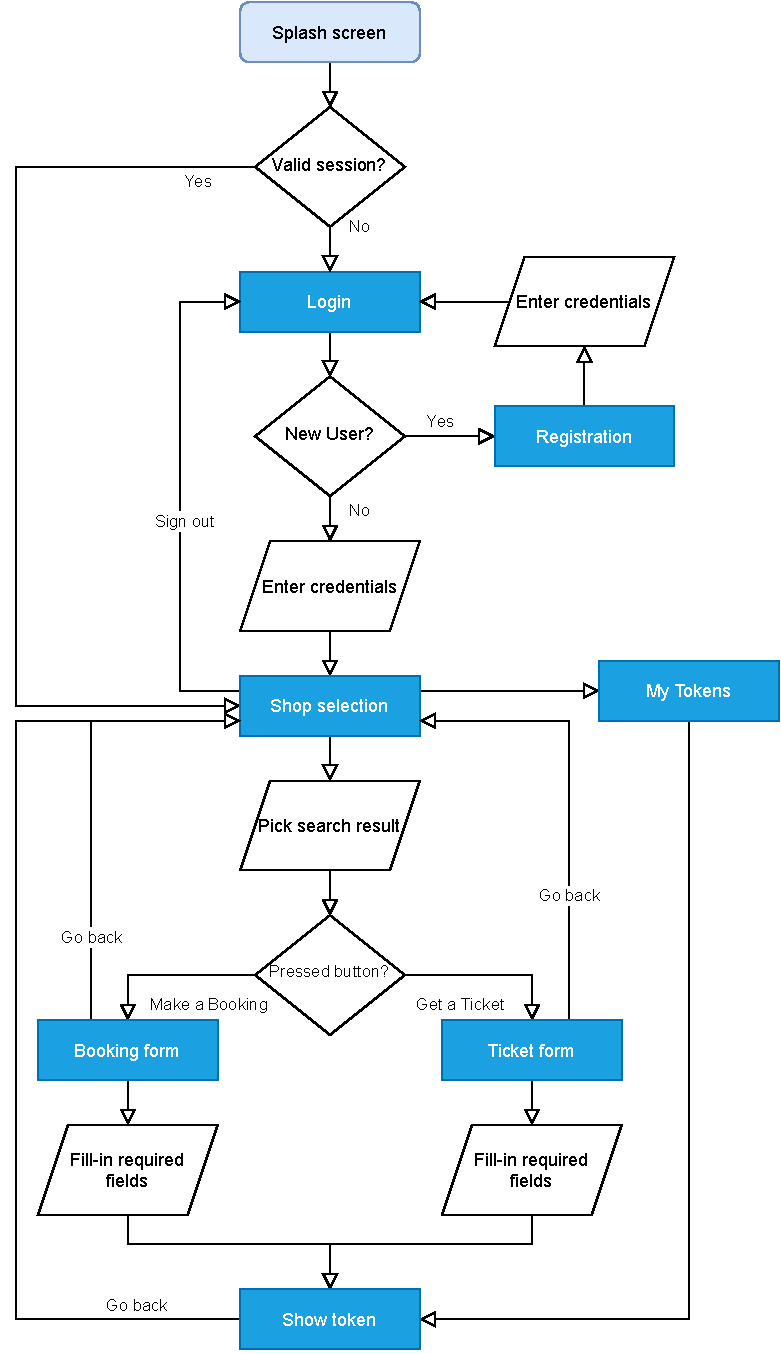
\includegraphics[height=0.85\textheight]{Images/ux-flowchart.pdf}
    \caption{UX flowchart for a Customer}
\end{figure}
\begin{figure}[H]
    \centering
    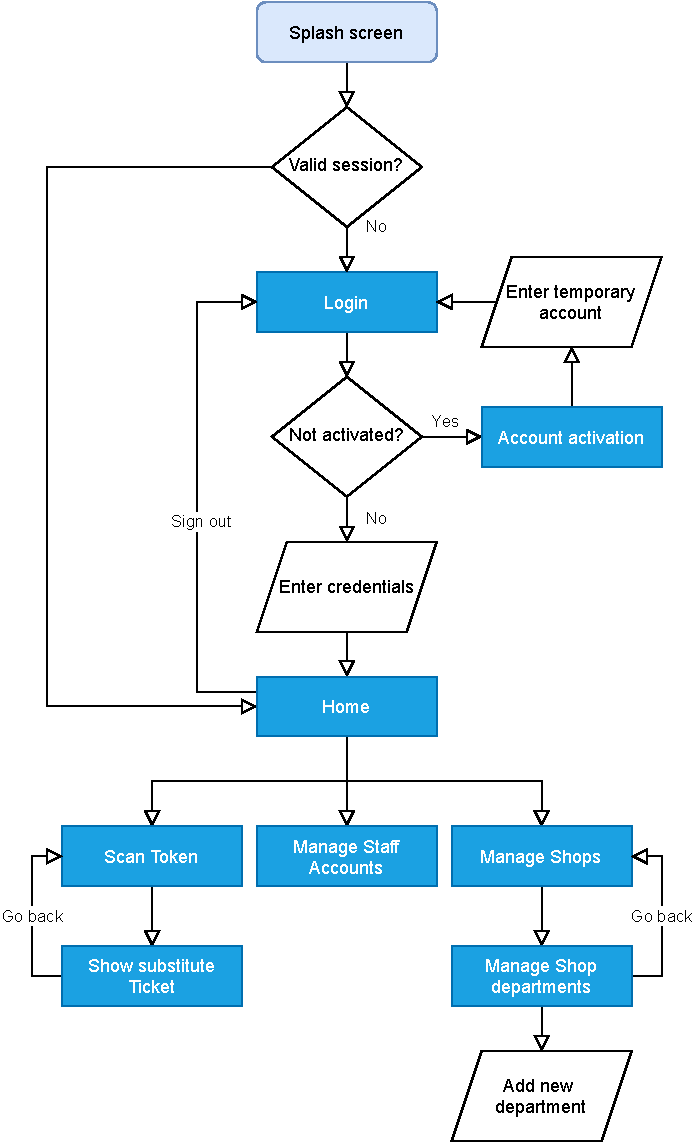
\includegraphics[height=0.85\textheight]{Images/ux-flowchart_staff.pdf}
    \caption{UX flowchart for a Staff member}
\end{figure}